\documentclass[12pt]{article}
\usepackage[T1]{fontenc}
\usepackage[T1]{polski}
\usepackage[utf8]{inputenc}
\newcommand{\BibTeX}{{\sc Bib}\TeX} 
\usepackage{graphicx}
\usepackage{amsfonts}
\usepackage{amsmath}
\usepackage{latexsym}
\usepackage{float}

\setlength{\textheight}{21cm}

\title{{\bf Zadanie nr 1 - Generacja sygnału i szumu}\linebreak
Cyfrowe Przetwarzanie Sygnałów}
\author{Dawid Jakubik, 224307 \and Hubert Gawłowski, 224298}
\date{22.04.2021}

\begin{document}
\clearpage\maketitle
\thispagestyle{empty}
\newpage
\setcounter{page}{1}
\section{Cel zadania}

Celem zadania było zapoznanie się z procesem konwersji A/C oraz C/A sygnałów jednocześnie poznając kilka metod na przeprowadzenie obu procesów jak i zaiplementowanie ich w aplikacji. 

\section{Wstęp teoretyczny}

Sygnały, które podlegaja kwantyzacji oraz rekonstrukcji generowane są na podstawie wzorów znajdujących się w instrukcji do zadania nr 1 \cite{instrukcja1}. W instrukcji \cite{instrukcji2} znajdują się wzory oraz opisy metod konwersji A/C oraz C/A użyte w celu kwantyzacji, rekonstrukcji oraz do obliczenia błędu średniokwadratowego, stosunku sygnał-szum, szczytowego stosunku sygnał-szum oraz maksymalnej różnicy.


\section{Eksperymenty i wyniki}

%%%%%%%%%%%%%%%%%%%%%%%%%%%%%%%%%%%%%%%%%%%%%%%%%%%%%%%%%%%%%%%%%%%%%%%%%%%%%%%%%%%%%%%%%%%%%%%%%%%%%%%%%%%%%%%%%
% PODROZDZIA£ PT. EKSPERYMENT NR 1 
%%%%%%%%%%%%%%%%%%%%%%%%%%%%%%%%%%%%%%%%%%%%%%%%%%%%%%%%%%%%%%%%%%%%%%%%%%%%%%%%%%%%%%%%%%%%%%%%%%%%%%%%%%%%%%%%%
W każdym z eksperymantów jako sygnał ciągły posłużył nam sygnał sinusoidalny o następujących parametrach: 
\begin{itemize}
	\item Amplituda: 4
	\item Czas początkowy: 0s
	\item Czas trwania sygnału: 2s
	\item Okres: 1s
\end{itemize}

\subsection{Eksperyment nr 1 Kwantyzacja równomierna z obcięciem}

Celem eksperymentu było przeprowadzenie kwantyzacji sygnału ciągłego z obcięciem.

\subsubsection{Założenia}

\begin{itemize}
    \item Częstotliwość próbkowania:
    \item Liczba bitów zapisu poziomów kwantyzacji:
\end{itemize}
\subsubsection{Przebieg}
Wygenerowany sygnał oraz jego skwantyzowana postać prezentują sie następująco:
\begin{figure}[H]
    \centering
    \includegraphics{cps_kwantyzacja_z_obcieciem.jpg}
    \caption{Kwantyzacja równomierna z obcięciem sygnału sinusoidalnego}
    \label{wykres dla eksperymentu 1}
\end{figure}

\subsubsection{Rezultat}
Obliczone miary dla procesu kwantyzacji:
\begin{figure}[H]
    \centering
    \includegraphics{cps_kwantyzacja_z_obcieciem_miary.jpg}
    \caption{Miary obliczone dla kwantyzacji równomiernej z obcięciem sygnału sinusoidalnego}
    \label{Wartości dla eksperymentu 1}
\end{figure}


%%%%%%%%%%%%%%%%%%%%%%%%%%%%%%%%%%%%%%%%%%%%%%%%%%%%%%%%%%%%%%%%%%%%%%%%%%%%%%%%%%%%%%%%%%%%%%%%%%%%%%%%%%%%%%%%%

%%%%%%%%%%%%%%%%%%%%%%%%%%%%%%%%%%%%%%%%%%%%%%%%%%%%%%%%%%%%%%%%%%%%%%%%%%%%%%%%%%%%%%%%%%%%%%%%%%%%%%%%%%%%%%%%%

\newpage
\subsection{Eksperyment nr 2 : Kwantyzacja równomierna z zaokrąglaniem}

Celem eksperymentu było przeprowadzenie kwantyzacji sygnału ciągłego z zaokrągleniem.

\subsubsection{Założenia}

\begin{itemize}
	\item Częstotliwość próbkowania:
	\item Liczba bitów zapisu poziomów kwantyzacji:
\end{itemize}
\subsubsection{Przebieg}
Wygenerowany sygnał oraz jego skwantyzowana postać prezentują sie następująco:
\begin{figure}[H]
	\centering
	\includegraphics{cps_kwantyzacja_z_zaokrągleniem.jpg}
	\caption{Kwantyzacja równomierna z zaokrągleniem sygnału sinusoidalnego}
	\label{wykres dla eksperymentu 2}
\end{figure}

\subsubsection{Rezultat}
Obliczone miary dla procesu kwantyzacji:
\begin{figure}[H]
	\centering
	\includegraphics{cps_kwantyzacja_z_zaokrągleniem_miary.jpg}
	\caption{Miary obliczone dla kwantyzacji równomiernej z zaokrągleniem sygnału sinusoidalnego}
	\label{Wartości dla eksperymentu 2}
\end{figure}


%%%%%%%%%%%%%%%%%%%%%%%%%%%%%%%%%%%%%%%%%%%%%%%%%%%%%%%%%%%%%%%%%%%%%%%%%%%%%%%%%%%%%%%%%%%%%%%%%%%%%%%%%%%%%%%%%

%%%%%%%%%%%%%%%%%%%%%%%%%%%%%%%%%%%%%%%%%%%%%%%%%%%%%%%%%%%%%%%%%%%%%%%%%%%%%%%%%%%%%%%%%%%%%%%%%%%%%%%%%%%%%%%%%
\newpage
\subsection{Eksperyment nr 3: Ekstrapolacja zerowego rzędu}

Eksperyment nr 3 polegał na ekstrapolacji zerowego rzędu spróbkowanego sygnału ciągłego.
\subsubsection{Założenia}
W eksperymencie impuls jednostkowy został wygenerowany dla następujących parametrów:
\begin{itemize}
    \item Amplituda 4
    \item Czas początkowy 1s
    \item Czas trwania 5s
    \item Częstotliwość 4 Hz
    \item Numer próbki, dla której następuje skok 12
\end{itemize}
\subsubsection{Przebieg}
Wygenerowany sygnał prezentuje się następująco:
\begin{figure}[H]
    \centering
    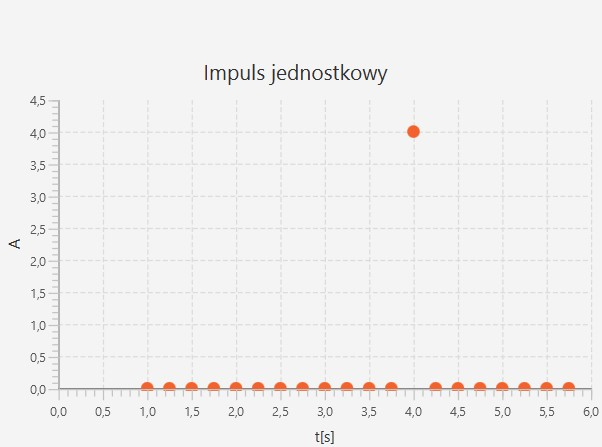
\includegraphics{cps_impuls_sygnal.jpg}
    \caption{Wykres impulsu jednostkowego dla parametrów:  A=1, t1=1s, d=5s, f=4Hz, ns=12}
    \label{wykres dla eksperymentu 3}
\end{figure}

Histogram dla powyższego impulsu wygląda następująco:
\begin{figure}[H]
    \centering
    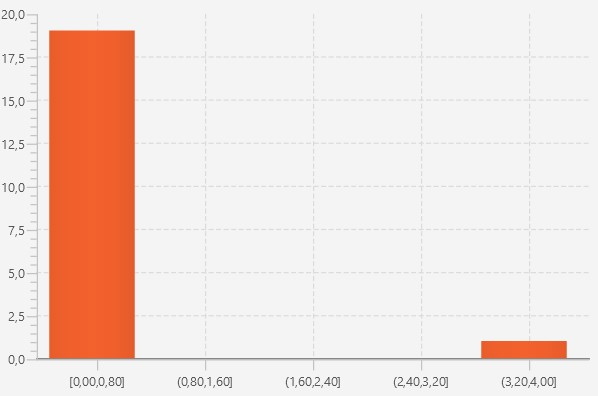
\includegraphics{cps_impuls_histogram.jpg}
    \caption{Histogram dla impulsu jednostkowego dla parametrów:  A=1, t1=1s, d=5s, f=4Hz, ns=12}
    \label{histogram dla eksperymentu 3}
\end{figure}


\subsubsection{Rezultat}
Obliczone parametry dla impulsu jednostkowego:
\begin{figure}[H]
    \centering
    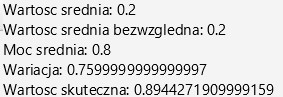
\includegraphics{cps_impuls_wartosci.jpg}
    \caption{Wartości obliczone dla impulsu jednostkowego dla parametrów:  A=1, t1=1s, d=5s, f=4Hz, ns=12}
    \label{wartości dla eksperymentu 3}
\end{figure}


%%%%%%%%%%%%%%%%%%%%%%%%%%%%%%%%%%%%%%%%%%%%%%%%%%%%%%%%%%%%%%%%%%%%%%%%%%%%%%%%%%%%%%%%%%%%%%%%%%%%%%%%%%%%%%%%%

%%%%%%%%%%%%%%%%%%%%%%%%%%%%%%%%%%%%%%%%%%%%%%%%%%%%%%%%%%%%%%%%%%%%%%%%%%%%%%%%%%%%%%%%%%%%%%%%%%%%%%%%%%%%%%%%%
\newpage
\subsection{Eksperyment nr 4: Interpolacja pierwszego rzędu}

Eksperyment nr 4 polegał na wygenerowaniu dwóch sygnałów (szumu gaussowskiego oraz sygnału sinusoidalnego) i dodaniu ich do siebie. Szum Gaussowski jest sygnałem którego amplituda przyjmuje losowe wartości z przedziału $<-A_{Gmax},A_{Gmax}>$ których rozkład prawdopodobieństwa jest rozkładem normalnym. Sygnał sinusoidalny opisuje funkcja:
\begin{equation}
    x(t)=Asin({2\PI}over{T}(t-t_1))
\end{equation}
\subsubsection{Założenia}
W eksperymencie szum został wygenerowany dla parametrów:
\begin{itemize}
    \item Amplituda: 0.1
    \item Czas początkowy: 0s
    \item Czas trwania sygnału: 2s
\end{itemize}
Sygnał sinusoidalny został wygenerowany dla parametrów:
\begin{itemize}
	\item Amplituda: 1
	\item Czas początkowy: 0s
	\item Czas trwania sygnału: 2s
	\item Okres: 1s
\end{itemize}
\begin{itemize}
    \item Amplituda: 1
    \item Czas początkowy: 0s
    \item Czas trwania sygnału: 2s
    \item Okres: 1s
\end{itemize}
\subsubsection{Przebieg}

W trakcie tego eksperymentu jako składniki dodawania wygenerowane zostały sygnały których wykresy, histogramy oraz obliczone wartości zostały pokazane na rysunkach od \ref{wykres dla sinusa} do \ref{wartosci dla szumu gausowskiego}
\begin{figure}[H]
    \centering
    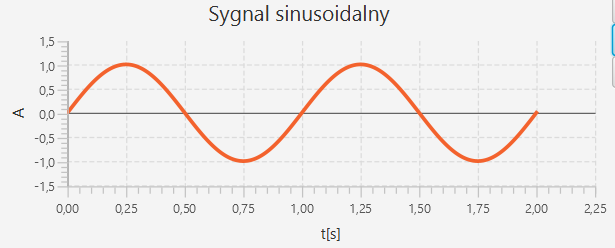
\includegraphics{cps_sinus_syg.PNG}
    \caption{Wykres sygnału sinusoidalnego dla parametrów:  A=1, t1=0s, d=1s, T=1s}
    \label{wykres dla sinusa}
\end{figure}
\begin{figure}[H]
    \centering
    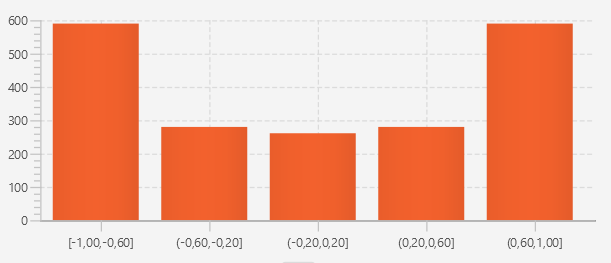
\includegraphics{cps_sinus_hist.PNG}
    \caption{Histogram sygnału sinusoidalnego dla parametrów:  A=1, t1=0s, d=1s, T=1s}
    \label{histogram dla sinusa}
\end{figure}
\begin{figure}[H]
    \centering
    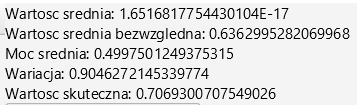
\includegraphics{cps_sinus_wart.PNG}
    \caption{Wartości obliczone dla sygnału sinusoidalnego dla parametrów:  A=1, t1=0s, d=1s, T=1s}
    \label{wartosci dla sinusa}
\end{figure}
\begin{figure}[H]
    \centering
    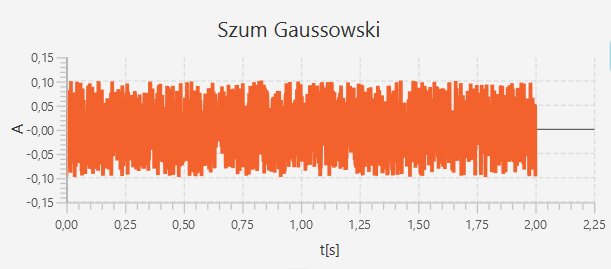
\includegraphics{cps_szum_gaussowski_syg.PNG}
    \caption{Wykres dla szumu gaussowskiego dla parametrów:  A=0.1, t1=0s, d=1s}
    \label{wykres dla szumu gausowskiego}
\end{figure}
\begin{figure}[H]
    \centering
    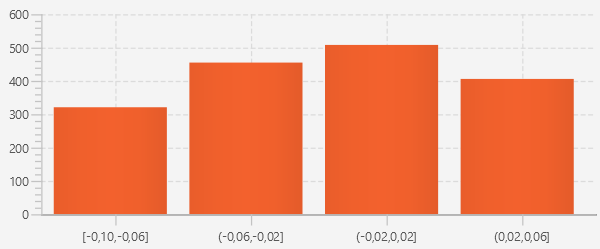
\includegraphics{cps_szum_gaussowski_hist.PNG}
    \caption{Histogram dla szumu gaussowskiego dla parametrów:  A=0.1, t1=0s, d=1s}
    \label{histogram dla szumu gausowskiego}
\end{figure}
\begin{figure}[H]
    \centering
    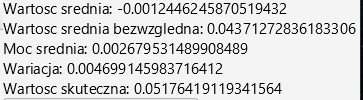
\includegraphics{cps_szum_gaussowski_wart.PNG}
    \caption{Wartości obliczone dla szumu gaussowskiego dla parametrów:  A=0.1, t1=0s, d=1s}
    \label{wartosci dla szumu gausowskiego}
\end{figure}

\subsubsection{Rezultat}
W wyniku dodania do siebie szumu gaussowskiego oraz sygnału sinusoidalnego otrzymaliśmy następujące wyniki:
\begin{figure}[H]
    \centering
    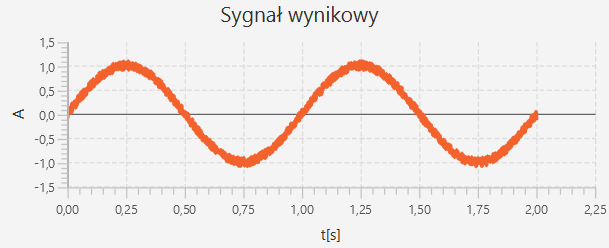
\includegraphics{cps_dodawanie_syg.PNG}
    \caption{Wartości obliczone dla sumy powyższych dwóch sygnałów}
    \label{wykres dodawania}
\end{figure}
\begin{figure}[H]
    \centering
    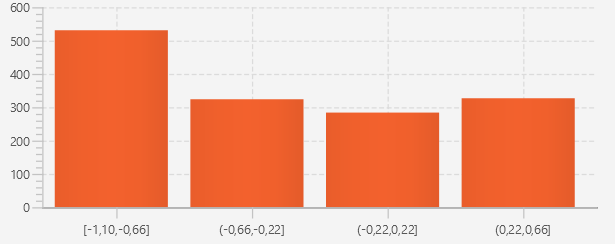
\includegraphics{cps_dodawanie_hist.PNG}
    \caption{Wartości obliczone dla sumy powyższych dwóch sygnałów}
    \label{histogram dodawania}
\end{figure}
\begin{figure}[H]
    \centering
    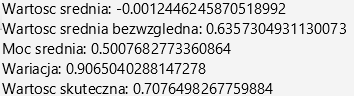
\includegraphics{cps_dodawanie_wart.PNG}
    \caption{Wartości obliczone dla sumy powyższych dwóch sygnałów}
    \label{wartosci dodawania}
\end{figure}


%%%%%%%%%%%%%%%%%%%%%%%%%%%%%%%%%%%%%%%%%%%%%%%%%%%%%%%%%%%%%%%%%%%%%%%%%%%%%%%%%%%%%%%%%%%%%%%%%%%%%%%%%%%%%%%%%

%%%%%%%%%%%%%%%%%%%%%%%%%%%%%%%%%%%%%%%%%%%%%%%%%%%%%%%%%%%%%%%%%%%%%%%%%%%%%%%%%%%%%%%%%%%%%%%%%%%%%%%%%%%%%%%%%
\newpage
\subsection{Eksperyment nr 5: Rekonstrukcja w oparciu o funkcję sinc 
 prostokątnego}
Eksperyment nr 5 polegał na wygenerowaniu dwóch sygnałów(sygnału sinusoidalnego wyprostowanego jednopołówkowo oraz sygnału prostokątnego) a następnie na obliczeniu różnicy tych sygnałów. Sygnał sinusoidalny wyprostowany jednopołówkowo posiada jedynie wartości nieujemne amplitudy i można opisać go funkcją:
\begin{equation}
    x(t)= 1 \over 2 A[sin({2\PI} \over {T} (t-t_1))+|sin({2\PI} \over {T} (t-t_1))|].
\end{equation}
Dla sygnału prostokątnego amplituda przyjmuje wartość zero lub $A_max$ i można go opisać wzorem:
\begin{equation}
    x(t)=\left\{\begin{matrix}A \: dla\: t\in \left \langle <kT+t_1, k_wT+kT+t_1)\right\\
    0 \: dla \: t\in \left \langle<k_wT-kT+t_1, T+kT+t_1\right\end{matrix} .\right
\end{equation}
\subsubsection{Założenia}
W eksperymencie sygnał sinusoidalny wyprostowany jednopołówkowo został wygenerowany dla parametrów:
\begin{itemize}
    \item Amplituda: 1
    \item Czas początkowy: 0s
    \item Czas trwania sygnału: 2s
    \item Okres: 1s
\end{itemize}
Sygnał prostokątny został wygenerowany dla parametrów:
\begin{itemize}
    \item Amplituda: 2
    \item Czas początkowy: 0s
    \item Czas trwania sygnału: 2s
    \item Okres: 1s
    \item Współczynnnik wypełnienia: 0.5
\end{itemize}
\subsubsection{Przebieg}
W trakcie tego eksperymentu wygenerowane zostały sygnały których wykresy, histogramy oraz obliczone wartości zostały pokazane na rysunkach od \ref{wykres dla sinusa jednopolowkowego} do \ref{wartosci dla prostokatnego}
\begin{figure}[H]
    \centering
    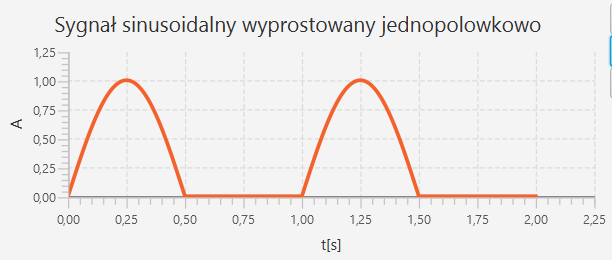
\includegraphics{cps_sinus_jednopolowkowy_syg.PNG}
    \caption{Wykres sygnału sinusoidalnego wyprostowanego jednopołówkowo dla parametrów:  A=1, t1=0s, d=2s, T=1s}
    \label{wykres dla sinusa jednopolowkowego}
\end{figure}
\begin{figure}[H]
    \centering
    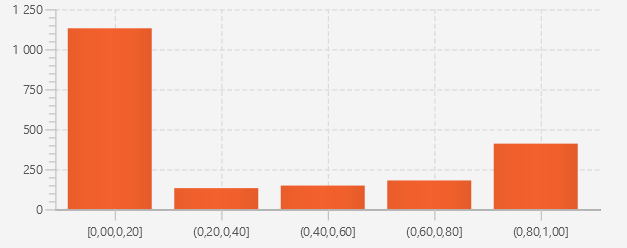
\includegraphics{cps_sinus_jednopolowkowy_hist.PNG}
    \caption{histogram sygnału sinusoidalnego wyprostowanego jednopołówkowo dla parametrów:  A=1, t1=0s, d=2s, T=1s}
    \label{histogram dla sinusa jednopolowkowego}
\end{figure}
\begin{figure}[H]
    \centering
    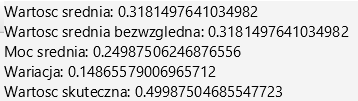
\includegraphics{cps_sinus_jednopolowkowy_wart.PNG}
    \caption{Wartości obliczone dla sygnału sinusoidalnego wyprostowanego jednopołówkowo dla parametrów:  A=1, t1=0s, d=2s, T=1s}
    \label{wartosci dla sinusa jednopolowkowego}
\end{figure}

\begin{figure}[H]
    \centering
    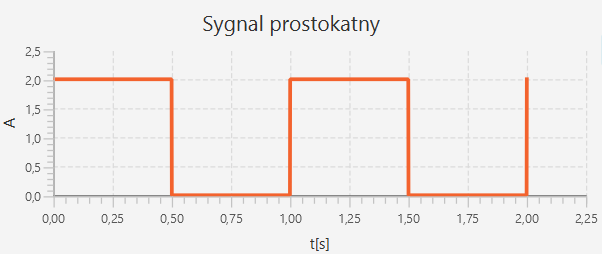
\includegraphics{cps_sygnal_prostokatny_syg.PNG}
    \caption{Wykres sygnału prostokątnego dla parametrów:  A=2, t1=0s, d=2s, T=1s, k_w=0.5}
    \label{wykres dla prostokatnego}
\end{figure}
\begin{figure}[H]
    \centering
    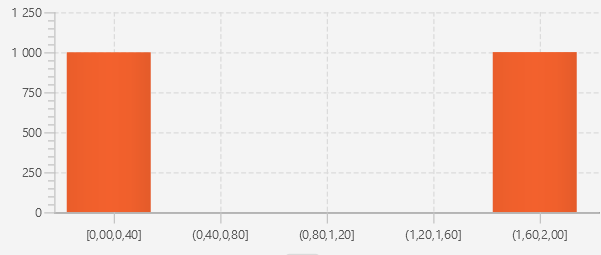
\includegraphics{cps_sygnal_prostokatny_hist.PNG}
    \caption{histogram sygnału prostokątnego dla parametrów:  A=2, t1=0s, d=2s, T=1s, k_w=0.5}
    \label{histogram dla prostokatnego}
\end{figure}
\begin{figure}[H]
    \centering
    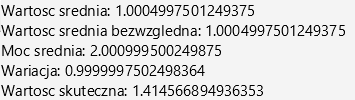
\includegraphics{cps_sygnal_prostokatny_wart.PNG}
    \caption{Wykres sygnału prostokątnego dla parametrów:  A=2, t1=0s, d=2s, T=1s, k_w=0.5}
    \label{wartosci dla prostokatnego}
\end{figure}
\subsubsection{Rezultat}
W wyniku odjęcia od sygnału sinusoidalnego wyprostowanego jednopołówkowo sygnału prostokątnego otrzymaliśmy widoczne poniżej wyniki.
\begin{figure}[H]
    \centering
    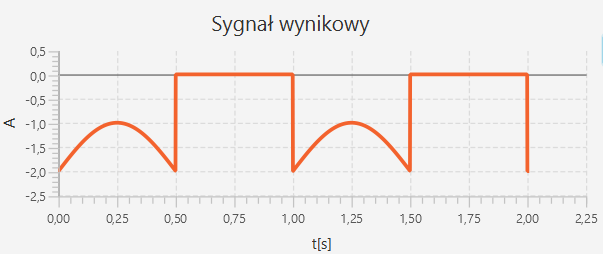
\includegraphics{cps_odejmowanie_syg.PNG}
    \caption{Wykres sygnału wynikowego operacji odejmowania}
    \label{wykres dla odejmowania}
\end{figure}
\begin{figure}[H]
    \centering
    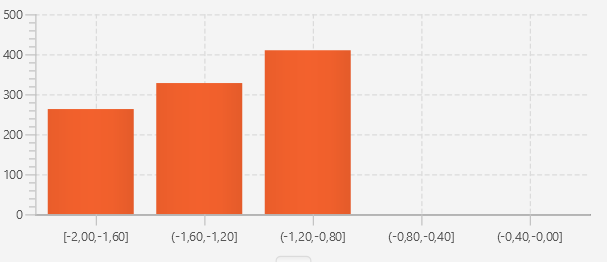
\includegraphics{cps_odejmowanie_hist.PNG}
    \caption{Histogram sygnału wynikowego operacji odejmowania}
    \label{histogram dla odejmowania}
\end{figure}
\begin{figure}[H]
    \centering
    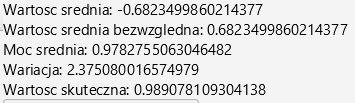
\includegraphics{cps_odejmowanie_wart.PNG}
    \caption{Wartości obliczone dla sygnału wynikowego operacji odejmowania}
    \label{wartosci dla odejmowania}
\end{figure}



%%%%%%%%%%%%%%%%%%%%%%%%%%%%%%%%%%%%%%%%%%%%%%%%%%%%%%%%%%%%%%%%%%%%%%%%%%%%%%%%%%%%%%%%%%%%%%%%%%%%%%%%%%%%%%%%%

%%%%%%%%%%%%%%%%%%%%%%%%%%%%%%%%%%%%%%%%%%%%%%%%%%%%%%%%%%%%%%%%%%%%%%%%%%%%%%%%%%%%%%%%%%%%%%%%%%%%%%%%%%%%%%%%%

\section{Wnioski}
\begin{itemize}
    \item Każdy sygnał ciągły można zdyskretyzować poprzez próbkowanie.
    \item Program poprawnie generuje zaimplementowane sygnały.
    \item Program pozwala na proste działania na sygnałach.
    \item Na podstawie histogramów w prosty sposób można dowiedzieć się o rozkładzie wartości.
\end{itemize}
 

%%%%%%%%%%%%%%%%%%%%%%%%%%%%%%%%%%%%%%%%%%%%%%%%%%%%%%%%%%%%%%%%%%%%%%%%%%%%%%%%%%%%%%%%%%%%%%%%%%%%%%%%%%%%%%%%%
% BIBLIOGRAFIA
%%%%%%%%%%%%%%%%%%%%%%%%%%%%%%%%%%%%%%%%%%%%%%%%%%%%%%%%%%%%%%%%%%%%%%%%%%%%%%%%%%%%%%%%%%%%%%%%%%%%%%%%%%%%%%%%%

\renewcommand\refname{Bibliografia}
\bibliographystyle{plain}
\bibliography{bibliografia_wzor}

\end{document}
